	\section {Introduction}\label{sec:introduction}

%	\footnoterule
%%	\footnotetext[1]{The work presented in this document corresponds to a review of the literature and a taxonomic proposal on virtual machines. This is the result of the inter-institutional effort between \textit{Universidad Tecnológica de Pereira, Pereira Colombia}, \textit{Universidad del Quindío, Armenia Colombia}, \textit{Universidad del Valle}, Cali Colombia, \textit{Universidad de Los Andes}, Bogotá Colombia and Clarkson University, Postdam, NY USA. This work is a part of the process of formation of the Doctorate in Engineering, emphasis in Computer Science of the Technological University of Pereira Colombia.}


	\footnotetext[1]{This is the result of the inter-institutional effort between \textit{Universidad Tecnol{\'o}gica de Pereira, Pereira Colombia}, \textit{Universidad del Quind{\'i}o, Armenia Colombia}, \textit{Universidad del Valle}, Cali Colombia, \textit{Universidad de Los Andes}, Bogot{\'a} Colombia and Clarkson University, Postdam, NY USA.}
	
%	\footnotetext[1]{The work presented in this document corresponds to a review of the literature and a taxonomic proposal on virtual machines. This is the result of the inter-institutional effort between \textit{Universidad Tecnol{\'o}gica de Pereira, Pereira Colombia}, \textit{Universidad del Quind{\'i}o, Armenia Colombia}, \textit{Universidad del Valle}, Cali Colombia, \textit{Universidad de Los Andes}, Bogot{\'a} Colombia and Clarkson University, Postdam, NY USA.} %This work is a part of the process of formation of the Doctorate in Engineering, emphasis in Computer Science of the Technological University of Pereira Colombia.}
	
	
	%JNM mostly edited to tighten up the sentences, remove words when the meaning is still clear without them
	%LESR - I agree
	In recent years virtualization technologies have been widely used to provide important benefits to organizations such as isolation, division of resources, consolidation, security, migration, and ease of administration \cite{Varasteh2017}.
	Virtualization also brings direct financial benefits to organizations in terms of return on investment (ROI), and reductions in the total cost of ownership (TCO) of the computer systems hardware \cite{Solis2014}, \cite{AbdElRahem2016}. Virtualization often provides substantial energy saving benefits as less energy is required to maintain a set of virtualized services that share fewer physical machines (server virtualization in data centers). This energy-saving aspect of virtualization is often called \textit{Green Computing} \cite {Thathera2015, Ranjith2017, Jing2011} and plays an important role in safeguarding the environment.	Other virtualization goals include increasing the scalability and availability of the computing environment and improvements to the administrative and security structures of the existing computational infrastructure \cite{Kusnetzky2011}, \cite{Hui2014}.
	
	%This involves the use of smaller amounts of energy to maintain operations related to information technology (IT), as is the case of server virtualization in data centers. 
	
	% Virtualization technologies have been able to consolidate mainly in the last two decades, \cite{Kampert2010}. 
	%This trend has led many organizations to start implementing these technologies, generating different types and approaches for the virtualization technologies developed. 
	 %Part of this situation is due to the fact that documents on technical procedures abound in the available documentation. 
	 %However, there are indeed fewer publications about the classification of virtualization types. 
	 %This situation makes it difficult to unify criteria on the denomination and the conceptual boundaries of the existing and emerging elements of this set of technologies.
	 
	%LESR - old - Before JNM
	
	%Virtualization technologies have revolutionized data centers in the last two decades, \cite{Kampert2010} and many variations of virtualization technologies have been developed. However in this vast and rapidly changing landscape of technologies offerings, there have been fewer publications on the classification of virtualization types. As virtualization technologies reach a level of maturity, we have an opportunity to look back and propose a set of criteria and boundaries to help explain and classify this set of technologies.
	

	%JNM Cubren 7 taxonomías diferentes. Creo que eso es mucho. En cambio, podría decir que ha habido varios intentos diferentes para una taxonomía y que este documento los revisa y compara y recomienda uno que aborde las debilidades en las taxonomías existentes.
	 
	%JNM - Muchas de mis ediciones son pequeñas sugerencias para reformular o enfocar el texto. Mi mayor sugerencia es ser muy claro sobre lo que es diferente en su nueva taxonomía. Este párrafo es un lugar perfecto para hacer eso.
	
	%JNM Enfatice aqui que está incluyendo las dos dimensiones principales ((Type of VM) and (Abstraction Level)) en un diagrama. 
	
	%LESR - old - Before JNM
	%%The previously published studies referenced in this document propose various taxonomies and models of existing virtualization technologies. 
	
	%JNM Si rellena esta frase me encantaría leer este parrafo otra vez.
	%In this paper, we present a taxonomy that improves and unifies previous work in X key ways: 1) and 2)....
	%I am not sure what you mean by "focus on the integration of resources"
	%Likewise, a taxonomy of virtual machines is proposed, which is focus on the integration of resources and combines different taxonomic studies. 
	
	%Relative to previous studies we also classify systems developed in more recent years.
	%We also include a taxonomic-key diagram that we believe will facilitate the selection of virtualization technologies based on our proposed taxonomy.
	
	%LESR - new
    The benefits of virtualization technologies have revolutionized data centers in the last two decades and have motivated the development of a number of variations in virtualization technologies \cite{Kampert2010} to suit different use cases.  In response, a number of attempts have been made in the academic literature to establish classification schemes for these variations of virtualization technologies.  In this document, we review these existing classification schemes and propose a revised taxonomy which responds to the several identified weaknesses in existing classification schemes. We summarize our classification approach with  a taxonomic-key diagram that can facilitate understanding and the selection of virtualization technologies for users. 
    
    
    %In this document, we include as elements to highlight: first a revision and compilation of classification schemes of virtual machines, second a new virtual machine taxonomy is proposed, which responds to the weaknesses found in the revised taxonomies, and finally includes a taxonomic key diagram, created to facilitate the selection of virtualization technologies according to the proposed new taxonomy. 
    
    %LESR - new
    
    
    The taxonomy that we present improves and unifies the previous work in classification of virtual machine technologies in the following three ways. First, we combine and unify approaches that consider both the virtual machine type  (Figure \ref{fig:twoApproaches}a) with approaches that consider the level of abstraction (Figure \ref{fig:twoApproaches}b). Second, we update classification approaches to include examples of virtualization technologies that have emerged more recently. Third, we introduce a taxonomic diagram based on our unified classification that can serve as a guide for selecting virtualization technologies in either academic or production environments.

%    \begin{center}
%		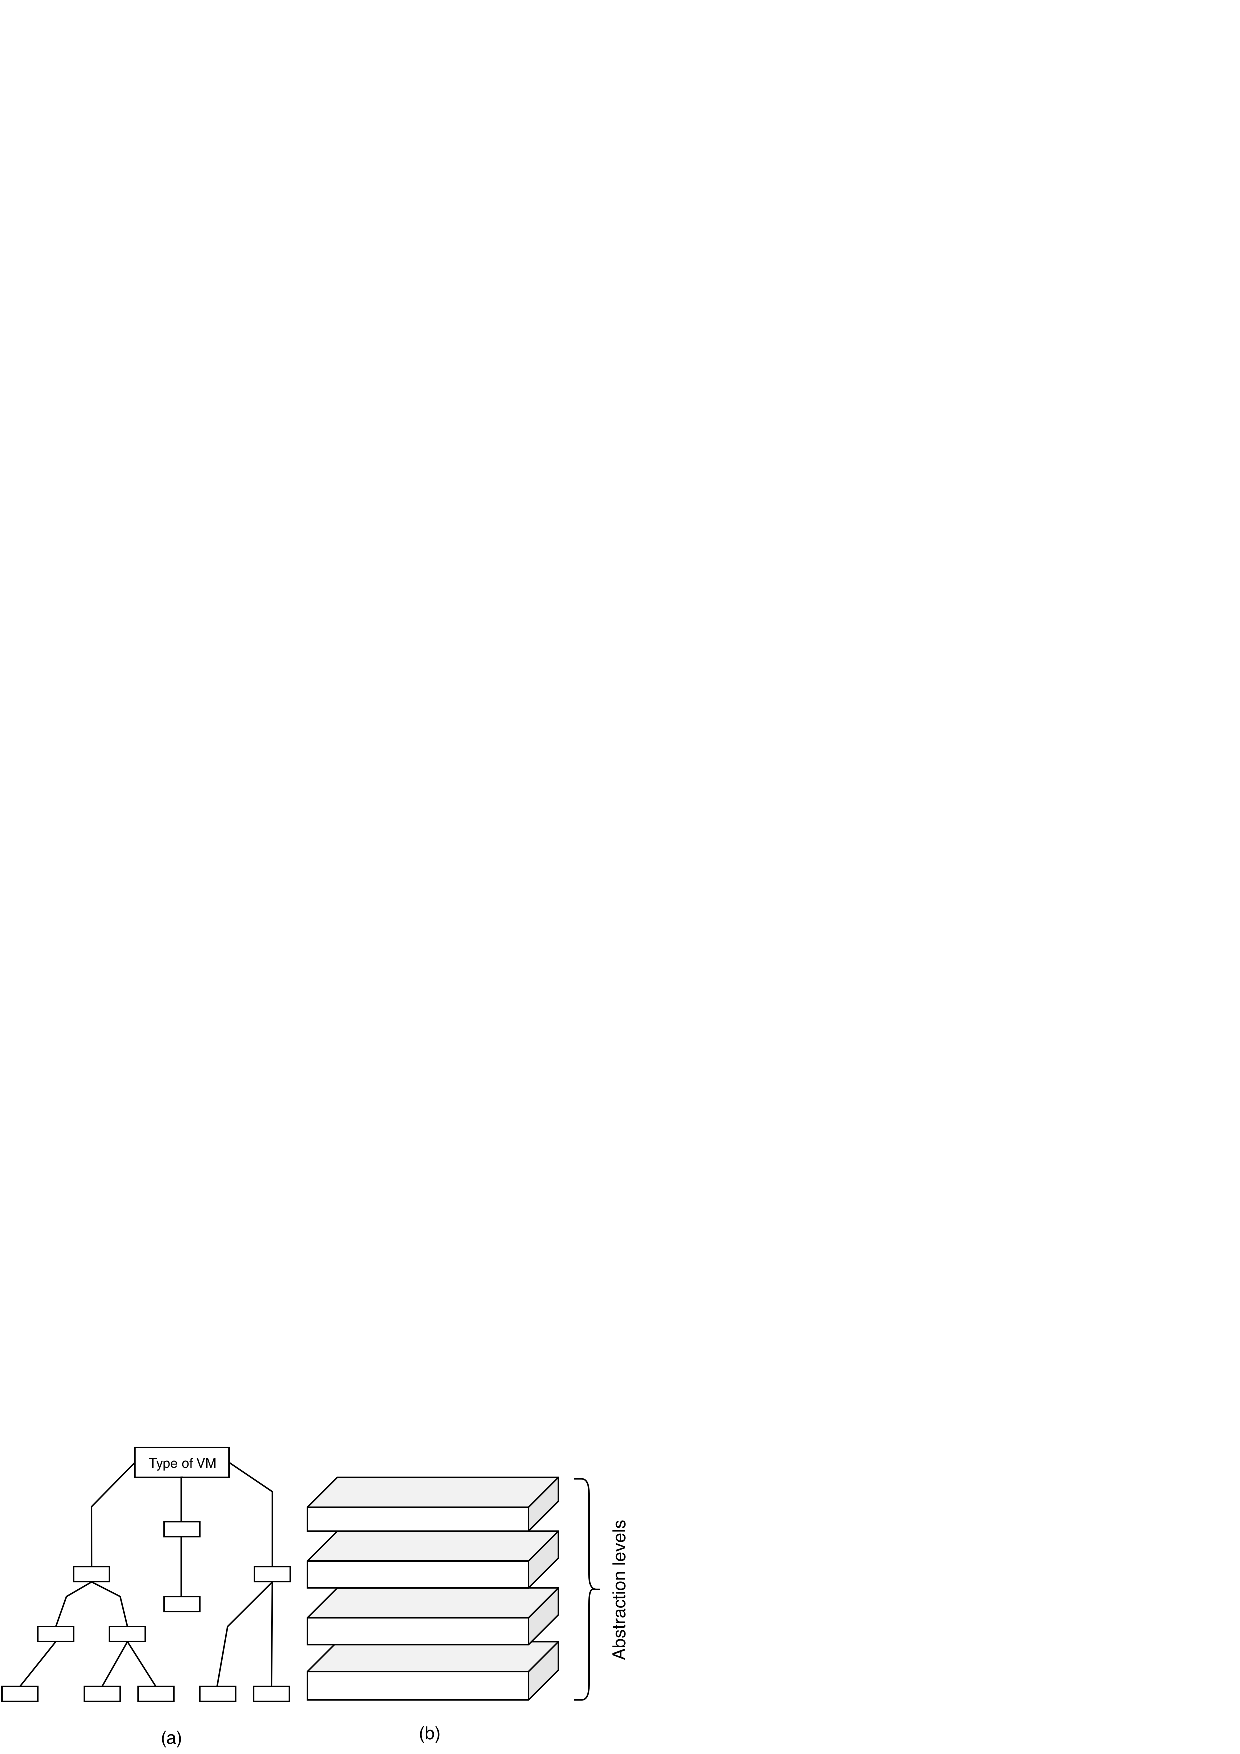
\includegraphics[width=8cm]{images/TwoApproaches.pdf}
%        %\vspace{1mm}
%        %\parbox[c]{8.3cm}{\footnotesize{Fig.1.~}  Example for inserting a one-column wide figure. }%\vspace*{.2mm}
%        \captionof{figure}{Two approaches used in the Taxonomy}
%        \label{fig:twoApproaches}
%    \end{center}

	\begin{figure}[H]
		\centering
		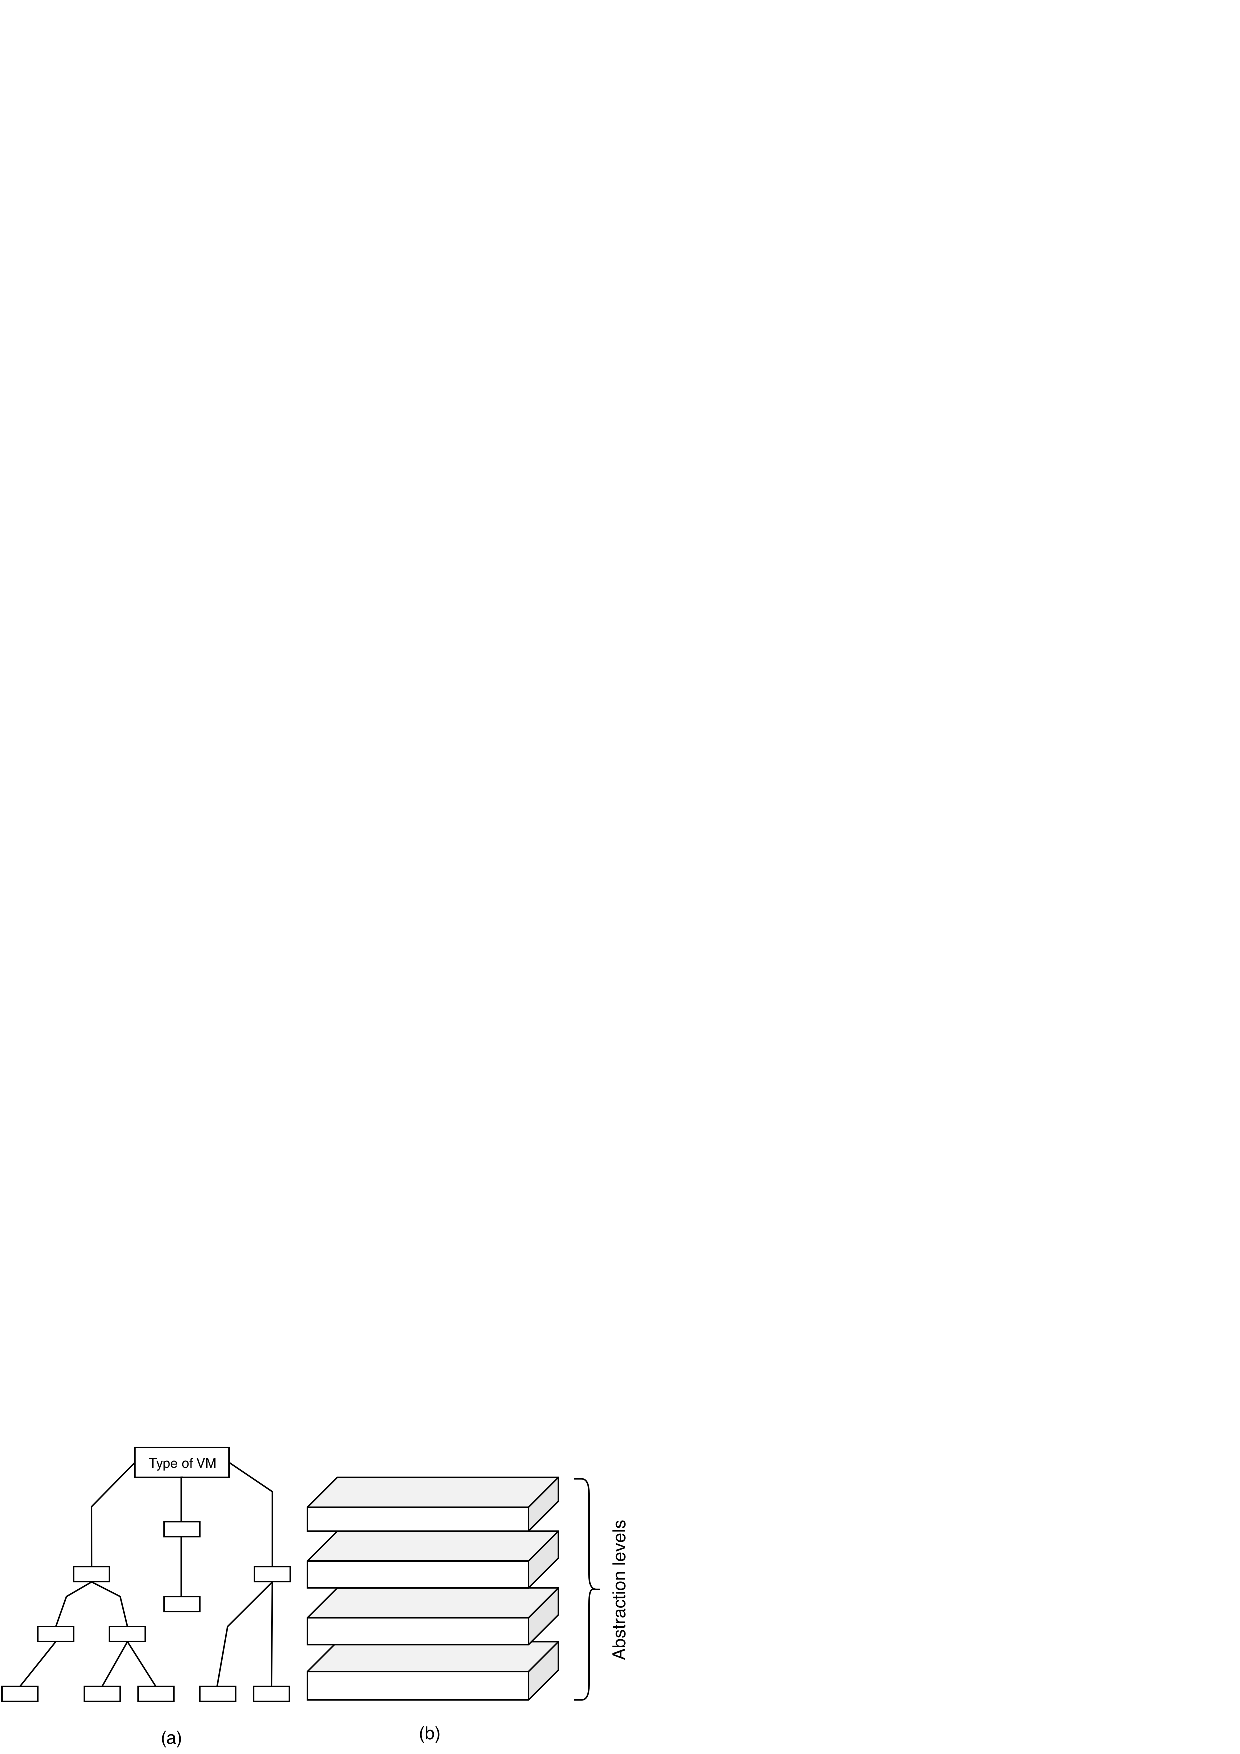
\includegraphics[width=8cm]{images/TwoApproaches.pdf}
		\vspace{-0.2cm}
		\caption{Two approaches used in the Taxonomy}
		\label{fig:twoApproaches}
	\end{figure}	
	
	The rest of the document is comprised of seven sections. Section \ref{sec:concetposVirtualizacion} introduces the basics of virtualization technologies.  Section \ref{sec:esquemasDeClasificacion} presents a description of previous classification schemes of virtualization technologies.  Section \ref{sec:necesidadDeUnaTaxonomia} describes the elements identified to propose a new taxonomy of virtual machines. Section \ref{sec:taxonomiaPropuesta} proposes a taxonomy that combines and updates the previous approaches. Section \ref{sec:choosingVirtualizationTechnology} presents a taxonomic diagram to guide the selection of the virtualization technologies identified in the proposed taxonomy.  Finally, Section \ref{sec:conclusion} presents our conclusions.
	